\documentclass[11pt]{article}

\usepackage[margin=0.85in]{geometry}
\usepackage[T1]{fontenc}
\usepackage{lmodern}
\usepackage{amsmath,amssymb}
\usepackage{enumitem}
\usepackage{hyperref}
\usepackage{xcolor}
\usepackage{booktabs}
\usepackage{array}
\usepackage{tikz}
\usepackage{float}
\usepackage{url}
\bibliographystyle{IEEEtran}

\usetikzlibrary{
    arrows.meta,
    positioning,
    calc,
    fit,
    backgrounds,
    shapes.geometric,
    shapes.multipart
}

\hypersetup{
    colorlinks=true,
    linkcolor=blue!50!black,
    urlcolor=blue!50!black
}

\setlist[itemize]{leftmargin=1.5em}
\setlist[enumerate]{leftmargin=1.8em}
\setlist[description]{
    leftmargin=0em,
    labelindent=0em,
    style=nextline,
    font=\normalfont
}

\tikzset{
    nnnode/.style={
        circle,
        draw=black!80,
        thick,
        fill=blue!8,
        minimum size=0.75cm,
        inner sep=1pt,
        font=\small
    },
    inputnode/.style={
        nnnode,
        fill=green!12
    },
    outputnode/.style={
        nnnode,
        fill=orange!15
    },
    hiddennode/.style={
        nnnode,
        fill=blue!10
    },
    connection/.style={
        -{Stealth[length=2mm]},
        thick,
        draw=black!75
    },
    newconnection/.style={
        -{Stealth[length=2mm]},
        very thick,
        draw=red!75!black
    },
    diagrambox/.style={
        draw=black!70,
        rounded corners=3pt,
        fill=gray!5,
        inner sep=7pt
    },
    workflowbox/.style={
        draw=black!75,
        rounded corners=3pt,
        fill=blue!5,
        align=center,
        minimum width=2.5cm,
        minimum height=0.9cm,
        font=\small
    },
    processbox/.style={
        draw=black!75,
        rounded corners=3pt,
        fill=green!7,
        align=center,
        minimum width=2.5cm,
        minimum height=0.9cm,
        font=\small
    },
    decisionbox/.style={
        diamond,
        draw=black!75,
        fill=orange!10,
        align=center,
        aspect=2,
        inner sep=2pt,
        font=\small
    },
    workflowarrow/.style={
        -{Stealth[length=2.2mm]},
        thick
    },
    optionalarrow/.style={
        -{Stealth[length=2.2mm]},
        thick,
        dashed
    }
}

\title{\textbf{NEAT: NeuroEvolution of Neural Network Topologies}}
\author{}
\date{}

\begin{document}

\maketitle

\tableofcontents

\newpage

% ============================================================
\section{Project Overview}
% ============================================================

This project implements a custom version of NeuroEvolution of Augmenting
Topologies (NEAT).

The implementation will support networks containing feedforward (FFNN),
recurrent (RNN), and long short-term memory (LSTM) cells. PyTorch will be
used for tensor operations and GPU acceleration, but its gradients and backpropagation will not be necessary for the genetic algorithm.

This project is designed to evolve a neural network (NN)for an arbitrary user defined simulation. The main test cases are pole balancing and maze solving.

% ============================================================
\section{Terminology}
% ============================================================

Here we define the common terms used for this project.

\begin{description}

    \item[\textbf{Tensor}]
    A tensor is a generalize array for numerical data, extending vectors and matrices to higher dimensions. This project uses PyTorch tensors
    to store and manipulate network weights and values over batches of agents. Tensor operations can be executed on a GPU, allowing
    many numerical operations to be performed in parallel.

    \item[\textbf{Network topology}]
    The network topology is the directed graph describing how information
    flows through a neural network. It consists of nodes and directed
    edges: nodes perform computations, while edges specify which nodes
    send information to which other nodes. The topology is distinct from
    the numerical weights stored on the edges. Two networks can have the
    same topology but different weights.

    \item[\textbf{Node / Cell}]
    A node, also called a cell in this project, is one computational unit
    in the network. It receives values from connected nodes, performs a
    computation, and produces an output. A cell can use different
    computational rules: an FFNN cell performs a feedforward operation,
    an RNN cell receives a hidden state between timesteps, and an LSTM
    cell maintains both a hidden state and a cell state.


    \item[\textbf{NEAT}]
    NeuroEvolution of Augmenting Topologies (NEAT) is an evolutionary
    algorithm that creates neural networks by evolving both their
    connection weights and their structures. NEAT maintains a population of candidate networks and
    improves them over generations using a survival of the fittest approach. Networks are evaluated in a task,
    better-performing networks are more likely to contribute to the
    next generation, and mutations can change weights or add and disable
    structural elements. This allows the algorithm to discover both
    network parameters and network topologies.

    \item[\textbf{Genome}]
    A genome is the description of one candidate neural
    network in NEAT. It contains the information describing its topology such as its nodes and
    connections, but also includes connection
    weights, enabled connections, and innovation numbers. The genome is
    the object that NEAT mutates, compares, and combines during evolution rather than operating directly on the compiled model itself.

    \item[\textbf{Gene}]
    A gene is one component of a genome that describes a particular part
    of the network. The gene contains the evolutionary information used by NEAT in addition to the model information. A genome is the collection of
    these genes that together describes an entire network. This implementation uses 2 genes: a node genes to describe
    individual nodes and connection genes to describe directed connections
    between nodes.

    \item[\textbf{Innovation number}]
    An innovation number is an identifier assigned to a
    structural change during evolution. When a mutation adds
    a connection, NEAT assigns that connection an innovation number. If
    the same structural mutation occurs independently in another genome,
    NEAT should recognize that to align the
    corresponding genes when comparing genomes or combining them during
    reproduction.

    \item[\textbf{Species}]
    A species is a group of genomes with sufficiently similar network
    structures. NEAT divides the population into species using a
    compatibility distance that measures structural and parameter
    differences between genomes. This grouping helps preserve diversity in different
    structural approaches: a newly developed network topology can compete
    primarily with similar networks rather than immediately being
    eliminated by a larger group of already well-performing networks.

    \item[\textbf{Population}]
    The population is the collection of genomes being evolved in one NEAT
    run. Each generation, the population's genomes are evaluated, assigned
    to species, and used to produce the next generation through selection,
    crossover, and mutation.

    \item[\textbf{Fitness}]
    Fitness is a numerical measure of how well a genome performs in the
    simulation task. The simulation calculates fitness from an agent's
    behavior.

    \item[\textbf{Batch}]
    In this project a batch does not refer to the training data samples being evaluated in parallel. Rather a batch is the collection of agents whose networks are evaluated
    together during a simulation run. Each agent is controlled by its own
    model, and the models may have different genomes and network
    topologies making gpu parallelization trickier. 

    \item[\textbf{Agent}]
    An agent is an individual entity acting within a simulation. It
    receives observations from the simulation, passes them to its assigned
    model, and uses the model's output as its action.

    \item[\textbf{State}]
    The set of information used to define the simulation at any given time. A simulation-state representation is not unique. The simulation-state can contain separate and additional information from the information fed to the model as observations.

    \item[\textbf{Model}]
    A model is an executable instance of a network described by a genome. Where as the genome is the evolutionary
    representation, while the model is the computational representation.

    \item[\textbf{Episode}]
    An episode is one complete evaluation of an agent in a simulation,
    beginning with a reset or initial state and ending when the agent
    terminates or reaches the simulation's time limit. A genome can be evaluated over multiple
    episodes using different initial conditions before its fitness is aggregated for evolution.


    \item[\textbf{Trajectory}]
    A trajectory is the list of an agent's simulation-state over an
    episode. It can be represented as a tensor with a state vector for multiple simulation timesteps, with an additional agent dimension
    when multiple agents are recorded together.

    \item[\textbf{Recurrent state}]
    Recurrent state is information retained by a model between timesteps.
    An FFNN has no recurrent state, an RNN retains a hidden state, and an
    LSTM retains both a hidden state and a cell state. This state allows
    a model to use information from earlier observations when producing
    its current action. Recurrent state is reset at the beginning of
    each episode.

    \item[\textbf{Crossover}]
    Crossover is the process of combining genes from two parent genomes
    to produce an offspring genome. NEAT uses innovation numbers to
    identify corresponding connection genes in the parents, allowing
    their network descriptions to be aligned even when their topologies
    differ.

    \item[\textbf{Mutation}]
    Mutation modifies a genome to create a new candidate network. Weight
    mutation changes numerical connection parameters, while structural
    mutations can add nodes or connections and disable existing
    connections.

\end{description}

% ============================================================
\subsection{Overview of NEAT}
% ============================================================

An example of a set of mutations to a given genome:


\begin{figure}[H]
\centering

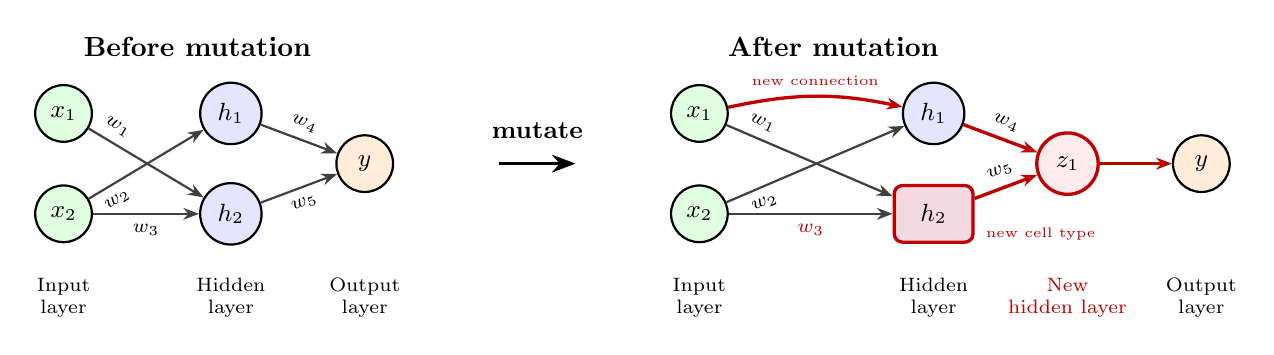
\begin{tikzpicture}[
    x=0.85cm,
    y=0.85cm,
    >=Stealth,
    every node/.style={font=\small},
    inputnode/.style={
        draw, circle, thick, fill=green!12,
        minimum size=0.72cm, inner sep=1pt
    },
    outputnode/.style={
        draw, circle, thick, fill=orange!15,
        minimum size=0.72cm, inner sep=1pt
    },
    ffnnnode/.style={
        draw, circle, thick, fill=blue!10,
        minimum size=0.78cm, inner sep=1pt
    },
    lstmnode/.style={
        draw=red!75!black, rounded corners=3pt, very thick, fill=purple!15,
        minimum width=1.0cm, minimum height=0.72cm,
        inner sep=2pt
    },
    newnode/.style={
        draw, circle, very thick,
        draw=red!75!black, fill=red!8,
        minimum size=0.78cm, inner sep=1pt
    },
    connection/.style={
        -{Stealth[length=2mm]},
        thick,
        draw=black!75
    },
    mutation/.style={
        -{Stealth[length=2mm]},
        very thick,
        draw=red!75!black
    }
]

% ============================================================
% Original network
% ============================================================

\node[font=\bfseries] at (-1.5,3.0) {Before mutation};

% Input layer
\node[inputnode] (x1a) at (-3.5,2) {$x_1$};
\node[inputnode] (x2a) at (-3.5,0.5) {$x_2$};

% Hidden layer: both cells are initially FFNN cells
\node[ffnnnode] (h1a) at (-1,2) {$h_1$};
\node[ffnnnode] (h2a) at (-1,0.5) {$h_2$};

% Output layer
\node[outputnode] (ya) at (1,1.25) {$y$};

% Existing connections
\draw[connection]
    (x1a) -- node[pos=0.18,above,sloped,font=\scriptsize] {$w_1$} (h2a);

\draw[connection]
    (x2a) -- node[pos=0.18,below,sloped,font=\scriptsize] {$w_2$} (h1a);

\draw[connection]
    (x2a) -- node[pos=0.5,below,sloped,font=\scriptsize] {$w_3$} (h2a);

\draw[connection]
    (h1a) -- node[above,sloped,font=\scriptsize] {$w_4$} (ya);

\draw[connection]
    (h2a) -- node[below,sloped,font=\scriptsize] {$w_5$} (ya);

% Layer labels
\node[font=\scriptsize,align=center] at (-3.5,-0.75)
    {Input \\ layer};

\node[font=\scriptsize,align=center] at (-1,-0.75)
    {Hidden \\ layer};

\node[font=\scriptsize,align=center] at (1,-0.75)
    {Output \\ layer};


% ============================================================
% Mutation transition
% ============================================================

\draw[-{Stealth[length=3mm]},very thick]
    (3.0,1.25) -- (4.15,1.25);

\node[font=\small\bfseries,align=center] at (3.58,1.75)
    {mutate};


% ============================================================
% Mutated network
% ============================================================

\node[font=\bfseries] at (8.0,3.0) {After mutation};

% Input layer
\node[inputnode] (x1b) at (6,2) {$x_1$};
\node[inputnode] (x2b) at (6,0.5) {$x_2$};

% Existing hidden layer
\node[ffnnnode] (h1b) at (9.5,2) {$h_1$};

% Cell-type mutation: FFNN -> LSTM
\node[lstmnode] (h2b) at (9.5,0.5) {$h_2$};
\node[font=\tiny,align=center,text=red!75!black] at (11.1,0.2)
    {new cell type};

% Newly added hidden layer, containing one node
\node[newnode] (z1b) at (11.5,1.25) {$z_1$};

% Output layer
\node[outputnode] (yb) at (13.5,1.25) {$y$};

% Original connections
\draw[connection]
    (x1b) -- node[pos=0.18,above,sloped,font=\scriptsize] {$w_1$} (h2b);

\draw[connection]
    (x2b) -- node[pos=0.18,below,sloped,font=\scriptsize] {$w_2$} (h1b);

\draw[connection]
    (x2b) -- node[pos=0.5,below,sloped,font=\scriptsize,text=red!75!black] {$w_3$} (h2b);


% Connection mutation: add x1 -> h1
\draw[mutation]
    (x1b) to[bend left=12]
    node[pos=0.5,above,sloped,font=\tiny,
         text=red!75!black] {new connection}
    (h1b);

% New hidden layer and its connections
\draw[mutation] (h1b) -- node[above,sloped,font=\scriptsize] {$w_4$} (z1b);
\draw[mutation] (h2b) -- node[above,sloped,font=\scriptsize] {$w_5$} (z1b);
\draw[mutation] (z1b) -- (yb);

% Layer labels
\node[font=\scriptsize,align=center] at (6,-0.75)
    {Input \\ layer};

\node[font=\scriptsize,align=center] at (9.5,-0.75)
    {Hidden \\ layer};

\node[font=\scriptsize,align=center,
      text=red!75!black] at (11.5,-0.75)
    {New \\ hidden layer};

\node[font=\scriptsize,align=center] at (13.5,-0.75)
    {Output \\ layer};

\end{tikzpicture}

\caption{A genome before and after three mutations: adding a
connection, changing an FFNN cell to an LSTM cell, and adding
a new hidden layer containing one node.}
\label{fig:genome-mutation}

\end{figure}



In this example each node and its connections are referred to as genes and their collection making up the topology and evolutionary state information is the genome.

This example shows the type of mutations possible: change weights, add or remove connections, add or remove nodes, add or remove layers, change cell type.

The mutation shown adds a new connection from \(x_1\) to \(h_2\). The
resulting genome has a different topology and therefore describes a
different network. The original genes are retained, while the new
connection is represented by an additional connection gene with its
own innovation number.

A wight update is a mutation a genome without changing its topology.

% ============================================================
\subsection{How NEAT Evolves Networks}
% ============================================================

NEAT evolves a population of genomes over multiple generations. Each
generation evaluates the current population, uses fitness to guide
reproduction, and produces a new population through crossover and
mutation.

\begin{figure}[H]
\centering

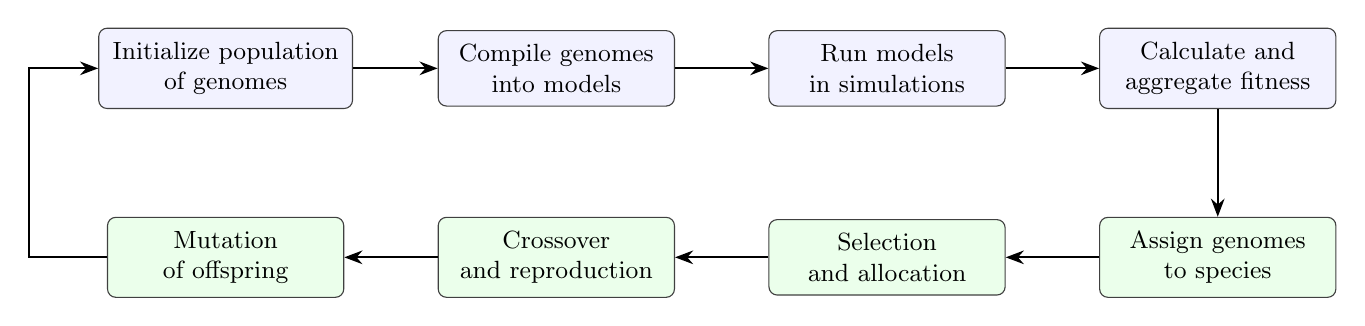
\begin{tikzpicture}[
    node distance=0.8cm and 0.9cm,
    every node/.style={font=\small},
    stage/.style={
        draw=black!75,
        rounded corners=3pt,
        fill=blue!5,
        align=center,
        minimum width=3.0cm,
        minimum height=0.9cm,
        inner sep=5pt
    },
    evolution/.style={
        draw=black!75,
        rounded corners=3pt,
        fill=green!8,
        align=center,
        minimum width=3.0cm,
        minimum height=0.9cm,
        inner sep=5pt
    },
    arrow/.style={
        -{Stealth[length=2.3mm]},
        thick
    }
]

% Main workflow, top row
\node[stage] (initialize) at (0,0)
    {Initialize population\\of genomes};

\node[stage] (compile) at (4.2,0)
    {Compile genomes\\into models};

\node[stage] (simulate) at (8.4,0)
    {Run models\\in simulations};

\node[stage] (fitness) at (12.6,0)
    {Calculate and\\aggregate fitness};

\draw[arrow] (initialize) -- (compile);
\draw[arrow] (compile) -- (simulate);
\draw[arrow] (simulate) -- (fitness);

% Evolutionary workflow, bottom row
\node[evolution] (speciate) at (12.6,-2.4)
    {Assign genomes\\to species};

\node[evolution] (selection) at (8.4,-2.4)
    {Selection\\and allocation};

\node[evolution] (reproduction) at (4.2,-2.4)
    {Crossover\\and reproduction};

\node[evolution] (mutation) at (0,-2.4)
    {Mutation\\of offspring};

\draw[arrow] (fitness) -- (speciate);
\draw[arrow] (speciate) -- (selection);
\draw[arrow] (selection) -- (reproduction);
\draw[arrow] (reproduction) -- (mutation);

% Return to next generation
\draw[arrow]
    (mutation.west) -- (-2.5,-2.4)
    -| (-2.5,-2.4)
    -- (-2.5,0.0)
    -| (-2.5,0.0)
    -- (initialize.west);

\end{tikzpicture}

\caption{Simplified NEAT evolutionary workflow. The top row shows
evaluation and fitness calculation. The bottom row shows how the
population is organized and how the next generation is produced.}
\label{fig:neat-workflow}
\end{figure}

The workflow steps are:

\begin{enumerate}
    \item \textbf{Initialize:} Create an initial population of genomes
    describing candidate neural networks.

    \item \textbf{Compile:} Convert each genome into an executable model.

    \item \textbf{Evaluate:} Run the models in the selected simulation.
    Each model controls an agent through one or more episodes.

    \item \textbf{Calculate fitness:} Use the simulation results to
    assign fitness to each genome. If a genome is evaluated over multiple
    episodes, its episode fitness values are aggregated.

    \item \textbf{Speciate:} Group structurally similar genomes into
    species using compatibility distance.

    \item \textbf{Select:} Allocate reproduction opportunities based
    on fitness, species performance, and the configured selection
    strategy.

    \item \textbf{Reproduce:} Create offspring by selecting parent
    genomes and combining their genes through crossover.

    \item \textbf{Mutate:} Modify offspring genomes through weight
    mutations and structural mutations.

    \item \textbf{Repeat:} Evaluate the resulting population as the
    next generation.
\end{enumerate}

This process repeats until a configured stopping condition is reached,
such as a maximum number of generations or a target fitness.

% ============================================================
\section{Project Structure}
% ============================================================

The project is organized into the following structure.

\begin{verbatim}
project/
    neat/
        neat.py
        genome.py
        genes.py
        innovation.py
        species.py

    models/
        model.py
        compiler.py
        cells.py

    simulations/
        simulation.py
        maze.py
        pole_balancing.py

    visualization/
        topology.py
        replay.py

    experiments/
        train.py
        evaluate.py
        configs/
\end{verbatim}

\subsection{NEAT Package}

\begin{description}

    \item[\textbf{\texttt{NEAT} -- \texttt{neat.py}}]
    \hspace{1em} Responsible for managing the population and evolution algorithm defining
    \texttt{initialize\_population()},
    \texttt{evaluate\_population()},
    \texttt{speciate()},
    \texttt{reproduce()}, and
    \texttt{evolve()}.

    \item[\textbf{\texttt{Genome} -- \texttt{genome.py}}]
    \hspace{1em}Stores the node and connection genes describing one
    candidate network. Implements structural and parameter mutation,
    crossover, compatibility distance, validation, and serialization.

    \item[\textbf{\texttt{NodeGene}, \texttt{ConnectionGene} -- \texttt{genes.py}}]
    \hspace{1em}Simple dataclass objects for storing individual nodes and
    connections information.

    \item[\textbf{\texttt{InnovationTracker} -- \texttt{innovation.py}}]
    \hspace{1em}Assigns and tracks historical innovation numbers so
    structural mutations can be identified consistently across genomes.

    \item[\textbf{\texttt{Species} -- \texttt{species.py}}]
    \hspace{1em}Maintains a group of structurally similar genomes,
    including its representative, membership, adjusted fitness, and
    stagnation information.

\end{description}

\subsection{Models Package}

\begin{description}

    \item[\textbf{\texttt{Model} -- \texttt{model.py}}]
    \hspace{1em}Represents an executable network compiled from a genome.
    Exposes the forward-pass interface and manages runtime recurrent
    state, including state reset between episodes.

    \item[\textbf{\texttt{Compiler} -- \texttt{compiler.py}}]
    \hspace{1em}Validates a genome and converts its graph representation
    into an execution plan. Determines a valid topological order,
    organizes connections, and prepares the tensor data required by
    execution.

    \item[\textbf{\texttt{Cells} -- \texttt{cells.py}}]
    \hspace{1em}Implements the tensor operations used to evaluate FFNN,
    RNN, and LSTM cells. Coordinates execution according to the
    compiled plan and supports batched evaluation where network
    structures are compatible.

\end{description}

\subsection{Simulations Package}

\begin{description}

    \item[\textbf{\texttt{Simulation} -- \texttt{simulation.py}}]
    \hspace{1em}Defines the common simulation interface and generic
    episode loop. Handles model execution, observations, actions,
    agent tracking, fitness accumulation, and optional recording. This is an abstract class that must be inherited with concrete implementations.

    \item[\textbf{\texttt{MazeSimulation} -- \texttt{maze.py}}]
    \hspace{1em}Implements the environment-specific behavior for maze
    navigation.

    \item[\textbf{\texttt{PoleBalancingSimulation} -- \texttt{pole\_balancing.py}}]
    \hspace{1em}Implements the environment-specific behavior for pole
    balancing.

\end{description}

\subsection{Visualization Package}

\begin{description}

    \item[\textbf{\texttt{TopologyVisualization} -- \texttt{topology.py}}]
    \hspace{1em}Plots a genome as a directed graph, showing nodes,
    connections, cell types, and optionally connection weights,
    innovation numbers, and disabled connections.

    \item[\textbf{\texttt{Replay} -- \texttt{replay.py}}]
    \hspace{1em}Loads a saved episode record and replays the agent's
    actions in the corresponding simulation. Replay uses the recorded
    actions rather than requiring the neural network to be executed again.

\end{description}

\subsection{Experiments Package}

The \texttt{experiments/} package contains entry points for training and
evaluating networks.

% ============================================================
\section{Genome Representation}
% ============================================================

A genome stores a network as a directed graph consisting of node genes
and connection genes. Each node has a unique identifier and a role.
Input and output nodes define the network interface and thus have more limited mutations allow on them, while hidden nodes perform computations and can experience any mutation.

Each node gene stores information such as:

\begin{quote}
\begin{itemize}
    \item A unique node identifier.
    \item Its role: input, hidden, or output.
    \item Its computational type: FFNN, RNN, or LSTM where applicable.
    \item Its activation function, where applicable.
    \item Any node-specific parameters, such as biases.
\end{itemize}
\end{quote}

Each connection gene stores information such as:

\begin{quote}
\begin{itemize}
    \item A unique connection identifier.
    \item Source and target node identifiers.
    \item Its weight or gate-specific weights.
    \item Whether the connection is enabled.
    \item Its innovation number.
\end{itemize}
\end{quote}

The genome is the evolutionary representation. This separation allows genomes to be mutated, compared,
serialized, and inspected independently of model execution.

% ============================================================
\section{Model Execution}
% ============================================================

Each node represents a
cell, and each directed connection specifies how information flows
between two cells. The compiler converts this graph into an execution
plan that can be evaluated using PyTorch tensors.

The initial implementation supports three cell types:

\begin{itemize}
    \item \textbf{FFNN:} A feedforward cell with no state carried between
    timesteps.
    \item \textbf{RNN:} A recurrent cell that retains a hidden state
    between timesteps.
    \item \textbf{LSTM:} A recurrent cell that retains both a hidden
    state and a cell state between timesteps.
\end{itemize}

The enabled feedforward connections must form a directed acyclic graph
(DAG). This allows the compiler to determine a topological execution
order. Connections may skip intermediate layers: a cell can receive
inputs from any earlier cell in the execution order, not only from the
immediately preceding layer.

Let \(P_j\) denote the set of predecessor cells connected to cell \(j\).
Let \(y_k^{(t)}\) be the output of predecessor \(k\) at timestep \(t\).

\subsection{Feedforward Cell}

A feedforward cell computes its output from the current outputs of its
predecessors:

\[
    y_j^{(t)}
    =
    f_j\left(
        \sum_{k \in P_j} w_{kj} y_k^{(t)} + b_j
    \right),
\]

where \(w_{kj}\) is the connection weight, \(b_j\) is the cell bias,
and \(f_j\) is the selected activation function.

A feedforward cell does not retain state between timesteps. Its output
depends only on the current timestep's inputs and the outputs of its
predecessors.

\subsection{Recurrent Cell}

A recurrent cell receives current-timestep contributions from its
predecessors and also uses its own previous hidden state:

\[
    h_j^{(t)}
    =
    f_j\left(
        \sum_{k \in P_j} w_{kj} y_k^{(t)}
        + u_j h_j^{(t-1)}
        + b_j
    \right).
\]

Here, \(h_j^{(t-1)}\) is the cell's hidden state from the previous
timestep, and \(u_j\) is its recurrent weight. The current output is

\[
    y_j^{(t)} = h_j^{(t)}.
\]

The hidden state is initialized when an episode begins and retained
while the episode runs. This allows the cell to incorporate information
from earlier observations even when that information is not present in
the current input.

\subsection{Long Short-Term Memory (LSTM) Cell}

An LSTM cell maintains two state variables: a hidden state \(h_t\) and
a cell state \(c_t\). Its input, forget, output, and candidate gates
each have separate incoming connection weights, recurrent coefficients,
and biases.

For an LSTM cell \(j\), the gate pre-activations are

\[
\begin{aligned}
    a_i^{(t)}
    &=
    \sum_{k \in P_j} w_{kj}^{(i)} y_k^{(t)}
    + u_i h^{(t-1)} + b_i, \\
    a_f^{(t)}
    &=
    \sum_{k \in P_j} w_{kj}^{(f)} y_k^{(t)}
    + u_f h^{(t-1)} + b_f, \\
    a_o^{(t)}
    &=
    \sum_{k \in P_j} w_{kj}^{(o)} y_k^{(t)}
    + u_o h^{(t-1)} + b_o, \\
    a_g^{(t)}
    &=
    \sum_{k \in P_j} w_{kj}^{(g)} y_k^{(t)}
    + u_g h^{(t-1)} + b_g.
\end{aligned}
\]

The gate activations are

\[
\begin{aligned}
    i_t &= \sigma(a_i^{(t)}), \\
    f_t &= \sigma(a_f^{(t)}), \\
    o_t &= \sigma(a_o^{(t)}), \\
    g_t &= \tanh(a_g^{(t)}).
\end{aligned}
\]

The cell and hidden states are updated as

\[
\begin{aligned}
    c_t &= f_t c_{t-1} + i_t g_t, \\
    h_t &= o_t \tanh(c_t).
\end{aligned}
\]

The LSTM cell's output is \(y_j^{(t)} = h_t\). The cell state provides
a separate memory pathway, while the gates control how information is
retained, added, and exposed through the hidden state.

\subsection{Batched Execution}

The simulation can evaluate multiple agents together. If a batch
contains \(B\) agents, their observations and compatible cell states
can be represented using tensors with a leading batch dimension. For
example, a batch of \(B\) agents with \(d\) input features has an
observation tensor of shape

\[
    X^{(t)} \in \mathbb{R}^{B \times d}.
\]

The execution engine applies the appropriate cell operations to the
agents in the batch. When agents have compatible network
structures, their computations can be grouped into tensor operations.
Different topologies or cell types may require separate execution
groups or other handling by the execution engine.

\subsection{Model State and Episode Reset}

A compiled model contains the network parameters and execution plan,
while its recurrent state is maintained separately as runtime data.
At the beginning of each episode, recurrent states are reset:

\[
    h^{(0)} = 0,
    \qquad
    c^{(0)} = 0,
\]

Skip connections are represented as ordinary feedforward connections.
They do not require a special node or cell type. The compiler must
aggregate contributions from all connected predecessors rather than
assuming that every cell receives data only from the immediately
preceding layer.

% ============================================================
\section{Simulation and Episode Evaluation}
% ============================================================

The base \texttt{Simulation} class provides a generic episode loop.
Environment-specific subclasses implement the operations that depend
on the simulation itself.

The generic loop performs the following steps:

\begin{enumerate}
    \item Reset the environment and the recurrent states of the models.
    \item Obtain observations for all active agents.
    \item Evaluate each model to produce an action.
    \item Apply the actions to the simulation.
    \item Update fitness and other metrics.
    \item Optionally record simulation data.
    \item Repeat until all agents have terminated or the time limit is
    reached.
    \item Finalize fitness, metrics, and optional trajectory data.
\end{enumerate}

The simulation interface should provide the following environment
operations:

\begin{description}

    \item[\texttt{reset(seed=None, initial\_states=None)}]
    \hspace{1em}Initialize the environment, optionally using a seed or
    supplied initial states.

    \item[\texttt{get\_observations()}]
    \hspace{1em}Return the observations supplied to the agents' models.

    \item[\texttt{step(actions, active\_mask)}]
    \hspace{1em}Advance the environment using the actions of agents that
    are still active.

    \item[\texttt{is\_done()}]
    \hspace{1em}Determine which agents have terminated.

    \item[\texttt{get\_record()}]
    \hspace{1em}Return the simulation-defined information to be stored
    by the trajectory recorder.

    \item[\texttt{evaluate()}]
    \hspace{1em}Return final fitness and metrics for each agent.

\end{description}

Agents may terminate at different timesteps. The simulation therefore
maintains an active-agent mask and prevents terminated agents from
continuing to affect the environment or their recurrent states.

A genome may be evaluated over multiple episodes, such as different
initial conditions or random seeds. NEAT aggregates the resulting
fitness values to determine the genome's fitness for that generation.
Whenever possible, genomes should be evaluated using equivalent
initial conditions so that fitness comparisons are fair.

% ============================================================
\section{Trajectory Recording and Replay}
% ============================================================

Three types of data should remain conceptually separate:

\begin{enumerate}
    \item \textbf{Environment state:} The complete internal state
    maintained by the simulation.
    \item \textbf{Observation:} The subset of information provided to
    the neural network at a given timestep.
    \item \textbf{Trajectory record:} The information selected for
    storage and later analysis or visualization.
\end{enumerate}

The simulation defines the contents of a record through
\texttt{get\_record()}. The default \texttt{set\_trajectory\_method()} must be overloaded by a child class to set more custom trajectory tracking logic.

The recorder should support the following policies:

\begin{itemize}
    \item \texttt{last}: retain only the final record.
    \item \texttt{all}: retain every timestep.
    \item \texttt{interval}: retain every \(N\)-th timestep.
    \item \texttt{custom}: use a user-provided callback or event condition.
\end{itemize}

Tracking is separate from trajectory recording. It is an opt-in feature
for selected agents that stores the initial simulation state and the
actions taken at each timestep. Optional observations or additional
state information may also be stored.

Replay uses the saved action sequence to advance the simulation from
its recorded initial state. This avoids requiring the original neural
network to be executed again.

% ============================================================
\section{Topology Visualization}
% ============================================================

The topology visualization module plots the given genome as a
directed graph. It should distinguish input, hidden, and output nodes,
and visually distinguish FFNN, RNN, and LSTM cells.

Connections should indicate their direction. Optional annotations
include connection weights, innovation numbers, and a disabled connection should not be vizualized as part of the topology.



% ============================================================
\section{API Reference}
% ============================================================

This section defines the planned public interfaces with expected input and output data types.

% ------------------------------------------------------------
\subsection{NEAT Package}
% ------------------------------------------------------------

\subsubsection{\texttt{neat/genome.py}}

\paragraph{\texttt{Genome}}

Stores the node and connection genes describing one candidate network.


\textbf{Signature:}
\begin{quote}
\begin{verbatim}
Genome(...)
\end{verbatim}
\end{quote}

\textbf{Arguments:}
\begin{quote}
\begin{itemize}
    \item \texttt{GenomeConfig}: instance of the GenomeConfig dataclass.
\end{itemize}
\end{quote}

\textbf{Returns:}
\begin{quote}
\begin{itemize}
    \item \texttt{Genome}: instance of the Genome class.
\end{itemize}
\end{quote}

\paragraph{\texttt{Genome.mutate()}}

Applies mutations to the genome.

\textbf{Signature:}
\begin{quote}
\begin{verbatim}
mutate(...)
\end{verbatim}
\end{quote}

\textbf{Arguments:}
\begin{quote}
\begin{itemize}
    \item \texttt{Self}: instance of the Genome class.
\end{itemize}
\end{quote}

\textbf{Returns:}
\begin{quote}
\begin{itemize}
    \item \texttt{Genome}: mutated instance of the Genome class.
\end{itemize}
\end{quote}

\paragraph{\texttt{Genome.crossover()}}

Combines genes from two parent genomes to produce an offspring genome.

\textbf{Signature:}
\begin{quote}
\begin{verbatim}
crossover(...)
\end{verbatim}
\end{quote}

\textbf{Arguments:}
\begin{quote}
\begin{itemize}
    \item \texttt{Genome}: instance of the Genome class.
    \item \texttt{Genome}: instance of the Genome class.
\end{itemize}
\end{quote}

\textbf{Returns:}
\begin{quote}
\begin{itemize}
    \item \texttt{Genome}: The offspring genome.
\end{itemize}
\end{quote}

\paragraph{\texttt{Genome.compatibility\_distance()}}

Calculates the compatibility distance between two genomes.

\textbf{Signature:}
\begin{quote}
\begin{verbatim}
compatibility_distance(...)
\end{verbatim}
\end{quote}

\textbf{Arguments:}
\begin{quote}
\begin{itemize}
    \item \texttt{Self}: instance of the Genome class.
    \item \texttt{Genome}: instance of the Genome class.
\end{itemize}
\end{quote}

\textbf{Returns:}
\begin{quote}
\begin{itemize}
    \item \texttt{TODO}: Compatibility distance.
\end{itemize}
\end{quote}

\paragraph{\texttt{Genome.validate()}}

Checks whether the genome satisfies the required structural constraints.

\textbf{Signature:}
\begin{quote}
\begin{verbatim}
validate(...)
\end{verbatim}
\end{quote}

\textbf{Arguments:}
\begin{quote}
\begin{itemize}
    \item \texttt{Self}: instance of the Genome class.
\end{itemize}
\end{quote}

\textbf{Returns:}
\begin{quote}
\begin{itemize}
    \item \texttt{Bool}: model constraint satisfaction.
\end{itemize}
\end{quote}

\paragraph{\texttt{Genome.serialize()}}

Converts the genome into a representation suitable for saving.

\textbf{Signature:}
\begin{quote}
\begin{verbatim}
serialize(...)
\end{verbatim}
\end{quote}

\textbf{Arguments:}
\begin{quote}
\begin{itemize}
    \item \texttt{Self}: instance of the Genome class.
\end{itemize}
\end{quote}

\textbf{Returns:}
\begin{quote}
\begin{itemize}
    \item \texttt{None}: Saves genome representation to a file.
\end{itemize}
\end{quote}

\paragraph{\texttt{GenomeConfig}}

Stores settings related to genome initialization and mutation.

\textbf{Constructor signature:}
\begin{quote}
\begin{verbatim}
GenomeConfig(...)
\end{verbatim}
\end{quote}

\textbf{Arguments:}
\begin{quote}
\begin{itemize}
    \item \texttt{Str|Path}: Configuration parameter json file.
\end{itemize}
\end{quote}

\textbf{Returns:}
\begin{quote}
\begin{itemize}
    \item \texttt{GenomeConfig}: A genome configuration instance.
\end{itemize}
\end{quote}


\subsubsection{\texttt{neat/genes.py}}

\paragraph{\texttt{NodeGene}}

Represents an individual node in a genome.

\textbf{Constructor signature:}
\begin{quote}
\begin{verbatim}
NodeGene(...)
\end{verbatim}
\end{quote}

\textbf{Arguments:}
\begin{quote}
\begin{itemize}
    \item \texttt{int}: Node identifier.
    \item \texttt{str}: Node role.
    \item \texttt{str}: Cell type.
    \item \texttt{function}: Activation function.
    \item \texttt{TODO}: Node-specific parameters.
\end{itemize}
\end{quote}

\textbf{Returns:}
\begin{quote}
\begin{itemize}
    \item \texttt{NodeGene}: A node gene instance.
\end{itemize}
\end{quote}

\paragraph{\texttt{ConnectionGene}}

Represents a directed connection between two nodes in a genome.

\textbf{Constructor signature:}
\begin{quote}
\begin{verbatim}
ConnectionGene(...)
\end{verbatim}
\end{quote}

\textbf{Arguments:}
\begin{quote}
\begin{itemize}
    \item \texttt{int}: Connection identifier.
    \item \texttt{int}: Source node identifier.
    \item \texttt{int}: Target node identifier.
    \item \texttt{tensor}: Connection weight(s).
    \item \texttt{bool}: Whether the connection is enabled.
    \item \texttt{int}: Innovation number.
\end{itemize}
\end{quote}

\textbf{Returns:}
\begin{quote}
\begin{itemize}
    \item \texttt{ConnectionGene}: A connection gene instance.
\end{itemize}
\end{quote}


\subsubsection{\texttt{neat/innovation.py}}

\paragraph{\texttt{InnovationTracker.get\_connection\_innovation()}}

Gets the innovation number associated with a structural connection mutation.

\textbf{Signature:}
\begin{quote}
\begin{verbatim}
get_connection_innovation(...)
\end{verbatim}
\end{quote}

\textbf{Arguments:}
\begin{quote}
\begin{itemize}
    \item \texttt{ConnectionGene}: Connection gene information.
\end{itemize}
\end{quote}

\textbf{Returns:}
\begin{quote}
\begin{itemize}
    \item \texttt{int}: Innovation number.
\end{itemize}
\end{quote}

\paragraph{\texttt{InnovationTracker.get\_node\_innovation()}}

Gets the innovation information associated with adding a node.

\textbf{Signature:}
\begin{quote}
\begin{verbatim}
get_node_innovation(...)
\end{verbatim}
\end{quote}

\textbf{Arguments:}
\begin{quote}
\begin{itemize}
    \item \texttt{NodeGene}: Node mutation identification information.
\end{itemize}
\end{quote}

\textbf{Returns:}
\begin{quote}
\begin{itemize}
    \item \texttt{int}: Node innovation information.
\end{itemize}
\end{quote}


\subsubsection{\texttt{neat/species.py}}

\paragraph{\texttt{Species.add()}}

Adds a genome to the species.

\textbf{Signature:}
\begin{quote}
\begin{verbatim}
add(...)
\end{verbatim}
\end{quote}

\textbf{Arguments:}
\begin{quote}
\begin{itemize}
    \item \texttt{Genome}: Genome to add.
\end{itemize}
\end{quote}

\textbf{Returns:}
\begin{quote}
\begin{itemize}
    \item \texttt{set[Genome]}: set of all genomes in the species.
\end{itemize}
\end{quote}

\paragraph{\texttt{Species.remove()}}

Removes a genome from the species.

\textbf{Signature:}
\begin{quote}
\begin{verbatim}
remove(...)
\end{verbatim}
\end{quote}

\textbf{Arguments:}
\begin{quote}
\begin{itemize}
    \item \texttt{Genome}: Genome to remove.
\end{itemize}
\end{quote}

\textbf{Returns:}
\begin{quote}
\begin{itemize}
    \item \texttt{set[Genome]}: set of all Genomes in the species.
\end{itemize}
\end{quote}


\subsubsection{\texttt{neat/neat.py}}

\paragraph{\texttt{NEAT.initialize\_population()}}

Creates the initial population of genomes.

\textbf{Signature:}
\begin{quote}
\begin{verbatim}
initialize_population(...)
\end{verbatim}
\end{quote}

\textbf{Arguments:}
\begin{quote}
\begin{itemize}
    \item \texttt{int}: seed.
\end{itemize}
\end{quote}

\textbf{Returns:}
\begin{quote}
\begin{itemize}
    \item \texttt{set[Genome]}: Initial population.
\end{itemize}
\end{quote}

\paragraph{\texttt{NEAT.evaluate\_population()}}

Evaluates the population using the selected simulation.

\textbf{Signature:}
\begin{quote}
\begin{verbatim}
evaluate_population(...)
\end{verbatim}
\end{quote}

\textbf{Arguments:}
\begin{quote}
\begin{itemize}
    \item \texttt{set[Genome]}: Population to evaluate.
\end{itemize}
\end{quote}

\textbf{Returns:}
\begin{quote}
\begin{itemize}
    \item \texttt{list[floats]}: Evaluation results or fitness values.
\end{itemize}
\end{quote}

\paragraph{\texttt{NEAT.speciate()}}

Assigns genomes to species based on compatibility distance.

\textbf{Signature:}
\begin{quote}
\begin{verbatim}
speciate(...)
\end{verbatim}
\end{quote}

\textbf{Arguments:}
\begin{quote}
\begin{itemize}
    \item \texttt{set[Genome]}: Population to assign to species.
\end{itemize}
\end{quote}

\textbf{Returns:}
\begin{quote}
\begin{itemize}
    \item \texttt{list[set[Genome]]}: Species assignments or updated species collection.
\end{itemize}
\end{quote}

\paragraph{\texttt{NEAT.reproduce()}}

Produces a new population through selection and reproduction.

\textbf{Signature:}
\begin{quote}
\begin{verbatim}
reproduce(...)
\end{verbatim}
\end{quote}

\textbf{Arguments:}
\begin{quote}
\begin{itemize}
    \item \texttt{int}: seed.
    \item \texttt{set[Genome]}: population to reproduce with.
\end{itemize}
\end{quote}

\textbf{Returns:}
\begin{quote}
\begin{itemize}
    \item \texttt{set[Genome]}: New population.
\end{itemize}
\end{quote}

\paragraph{\texttt{NEAT.evolve()}}

Runs the evolutionary process over multiple generations.

\textbf{Signature:}
\begin{quote}
\begin{verbatim}
evolve(...)
\end{verbatim}
\end{quote}

\textbf{Arguments:}
\begin{quote}
\begin{itemize}
    \item \texttt{int}: seed.
    \item \texttt{int}: max number of generations to run.
    \item \texttt{patience}: max number of generations to run without improvement on fitness score.
\end{itemize}
\end{quote}

\textbf{Returns:}
\begin{quote}
\begin{itemize}
    \item \texttt{None}: results are saved as files.
\end{itemize}
\end{quote}


\paragraph{\texttt{NEAT.evolve()}}

Runs the evolutionary process over multiple generations.

\textbf{Signature:}
\begin{quote}
\begin{verbatim}
evolve(...)
\end{verbatim}
\end{quote}

\textbf{Arguments:}
\begin{quote}
\begin{itemize}
    \item \texttt{int}: seed.
    \item \texttt{int}: max number of generations to run.
    \item \texttt{patience}: max number of generations to run without improvement on fitness score.
\end{itemize}
\end{quote}

\textbf{Returns:}
\begin{quote}
\begin{itemize}
    \item \texttt{None}: results are saved as files.
\end{itemize}
\end{quote}

% ------------------------------------------------------------
\subsection{Models Package}
% ------------------------------------------------------------

\subsubsection{\texttt{models/model.py}}

\paragraph{\texttt{Model.forward()}}

Evaluates the network for the supplied observations.

\textbf{Signature:}
\begin{quote}
\begin{verbatim}
forward(...)
\end{verbatim}
\end{quote}

\textbf{Arguments:}
\begin{quote}
\begin{itemize}
    \item \texttt{Tensor}: the simulation observations for a single model at a given timestep.
\end{itemize}
\end{quote}

\textbf{Returns:}
\begin{quote}
\begin{itemize}
    \item \texttt{Tensor}: Model's selected action.
\end{itemize}
\end{quote}

\paragraph{\texttt{Model.reset\_state()}}

Resets the recurrent state of the model.

\textbf{Signature:}
\begin{quote}
\begin{verbatim}
reset_state(...)
\end{verbatim}
\end{quote}

\textbf{Arguments:}
\begin{quote}
\begin{itemize}
    \item \texttt{None}: None
\end{itemize}
\end{quote}

\textbf{Returns:}
\begin{quote}
\begin{itemize}
    \item \texttt{None}: None
\end{itemize}
\end{quote}

\subsubsection{\texttt{models/compiler.py}}

\paragraph{\texttt{compile\_genome()}}

Compiles a genome into an executable model.

\textbf{Signature:}
\begin{quote}
\begin{verbatim}
compile_genome(...)
\end{verbatim}
\end{quote}

\textbf{Arguments:}
\begin{quote}
\begin{itemize}
    \item \texttt{genome}: Genome to compile.
\end{itemize}
\end{quote}

\textbf{Returns:}
\begin{quote}
\begin{itemize}
    \item \texttt{Model}: instance of the Model class.
\end{itemize}
\end{quote}

\paragraph{\texttt{validate\_topology()}}

Checks whether a genome's topology can be compiled.

\textbf{Signature:}
\begin{quote}
\begin{verbatim}
validate_topology(...)
\end{verbatim}
\end{quote}

\textbf{Arguments:}
\begin{quote}
\begin{itemize}
    \item \texttt{Genome}: Genome whose topology is being checked.
\end{itemize}
\end{quote}

\textbf{Returns:}
\begin{quote}
\begin{itemize}
    \item \texttt{Bool}: Topology validation result.
\end{itemize}
\end{quote}


\subsubsection{\texttt{models/cells.py}}

\paragraph{Cell operations}

This module implements the tensor operations for FFNN, RNN, and LSTM
cells. The specific function names and signatures are \texttt{TODO}.

% ------------------------------------------------------------
\subsection{Simulations Package}
% ------------------------------------------------------------

\subsubsection{\texttt{simulations/simulation.py}}

\paragraph{\texttt{Simulation.reset()}}

Initializes or resets the simulation.

\textbf{Signature:}
\begin{quote}
\begin{verbatim}
reset(...)
\end{verbatim}
\end{quote}

\textbf{Arguments:}
\begin{quote}
\begin{itemize}
    \item \texttt{int}: seed.
\end{itemize}
\end{quote}

\textbf{Returns:}
\begin{quote}
\begin{itemize}
    \item \texttt{None}: None.
\end{itemize}
\end{quote}

\paragraph{\texttt{Simulation.get\_observations()}}

Returns the observations supplied to the agents' models.

\textbf{Signature:}
\begin{quote}
\begin{verbatim}
get_observations(...)
\end{verbatim}
\end{quote}

\textbf{Arguments:}
\begin{quote}
\begin{itemize}
    \item \texttt{Tensor}: state of the current simulation for a given model.
\end{itemize}
\end{quote}

\textbf{Returns:}
\begin{quote}
\begin{itemize}
    \item \texttt{Tensor}: Observations for the given model's simulation.
\end{itemize}
\end{quote}

\paragraph{\texttt{Simulation.step()}}

Advances the simulation using the agents' actions.

\textbf{Signature:}
\begin{quote}
\begin{verbatim}
step(...)
\end{verbatim}
\end{quote}

\textbf{Arguments:}
\begin{quote}
\begin{itemize}
    \item \texttt{Tensor}: Actions produced by the agents' models.
\end{itemize}
\end{quote}

\textbf{Returns:}
\begin{quote}
\begin{itemize}
    \item \texttt{None}: updates the given's model simulation.
\end{itemize}
\end{quote}

\paragraph{\texttt{Simulation.is\_done()}}

Determines whether agents or the simulation have terminated.

\textbf{Signature:}
\begin{quote}
\begin{verbatim}
is_done(...)
\end{verbatim}
\end{quote}

\textbf{Arguments:}
\begin{quote}
\begin{itemize}
    \item \texttt{int}: target Model instance's id in the simulation's set of models.
\end{itemize}
\end{quote}

\textbf{Returns:}
\begin{quote}
\begin{itemize}
    \item \texttt{Bool}: Termination status.
\end{itemize}
\end{quote}

\paragraph{\texttt{Simulation.evaluate()}}

Calculates the fitness and any additional metrics for the agents.

\textbf{Signature:}
\begin{quote}
\begin{verbatim}
evaluate(...)
\end{verbatim}
\end{quote}

\textbf{Arguments:}
\begin{quote}
\begin{itemize}
    \item \texttt{Tensor}: A given genome's simulation trajectory vector.
\end{itemize}
\end{quote}

\textbf{Returns:}
\begin{quote}
\begin{itemize}
    \item \texttt{Float}: Fitness score.
\end{itemize}
\end{quote}

\paragraph{\texttt{Simulation.run\_sim()}}

Runs a simulation episode using the supplied models.

\textbf{Signature:}
\begin{quote}
\begin{verbatim}
run_sim(...)
\end{verbatim}
\end{quote}

\textbf{Arguments:}
\begin{quote}
\begin{itemize}
    \item \texttt{set[Genome]}: Models or agents to evaluate.
    \item \texttt{TODO}: Episode configuration.
\end{itemize}
\end{quote}

\textbf{Returns:}
\begin{quote}
\begin{itemize}
    \item \texttt{list[float]}: Episode evaluation results.
\end{itemize}
\end{quote}

\paragraph{\texttt{Simulation.set\_trajectory\_method()}}

Sets the policy used to record simulation trajectory data.

\textbf{Signature:}
\begin{quote}
\begin{verbatim}
set_trajectory_method(...)
\end{verbatim}
\end{quote}

\textbf{Arguments:}
\begin{quote}
\begin{itemize}
    \item \texttt{str|function}: Trajectory recording policy (last, all, step, custom).
\end{itemize}
\end{quote}

\textbf{Returns:}
\begin{quote}
\begin{itemize}
    \item \texttt{None}: None.
\end{itemize}
\end{quote}

\paragraph{\texttt{Simulation.get\_trajectory()}}

Returns the trajectory data recorded by the simulation.

\textbf{Signature:}
\begin{quote}
\begin{verbatim}
get_trajectory(...)
\end{verbatim}
\end{quote}

\textbf{Arguments:}
\begin{quote}
\begin{itemize}
    \item \texttt{int}: The target Model's id.
\end{itemize}
\end{quote}

\textbf{Returns:}
\begin{quote}
\begin{itemize}
    \item \texttt{TODO}: Recorded trajectory.
\end{itemize}
\end{quote}

% ------------------------------------------------------------
\subsection{Visualization Package}
% ------------------------------------------------------------

\subsubsection{\texttt{visualization/topology.py}}

\paragraph{\texttt{plot\_genome()}}

Plots a genome as a directed graph.

\textbf{Signature:}
\begin{quote}
\begin{verbatim}
plot_genome(...)
\end{verbatim}
\end{quote}

\textbf{Arguments:}
\begin{quote}
\begin{itemize}
    \item \texttt{genome}: Genome to visualize.
    \item \texttt{TODO}: Optional visualization settings.
\end{itemize}
\end{quote}

\textbf{Returns:}
\begin{quote}
\begin{itemize}
    \item \texttt{TODO}: Plot or visualization object.
\end{itemize}
\end{quote}


\subsubsection{\texttt{visualization/replay.py}}

\paragraph{Replay function(s)}

Replays a recorded simulation trajectory.

\textbf{Signature:}
\begin{quote}
\begin{verbatim}
TODO
\end{verbatim}
\end{quote}

\textbf{Arguments:}
\begin{quote}
\begin{itemize}
    \item \texttt{Simulation}: Simulation instance.
    \item \texttt{Tensor}: Recorded trajectory or replay data.
    \item \texttt{TODO}: Optional replay settings.
\end{itemize}
\end{quote}

\textbf{Returns:}
\begin{quote}
\begin{itemize}
    \item \texttt{TODO}: TODO.
\end{itemize}
\end{quote}


% ============================================================
% References
% ============================================================

\clearpage
\phantomsection
\addcontentsline{toc}{section}{References}

\nocite{*}
\bibliography{references}

\end{document}